\chapter{Conceptual foundations}
\label{chapter:conceptualFoundations}

\section{Telepresence}

The term Telepresence first appears in an article by Marvin Minsky in which the author roughly defines it as a form of remote robotic operation, that \textquote{emphasises the importance of high‑quality sensory feedback} and that its development's biggest challenge is \textquote{achieving that sense of \textquote{being there.}} \parencite{minskyTelepresence}. Minsky argued from a standpoint concerned mostly with robotic manipulators that performed labour either mediated over a distance or enhanced both the operator's abilities and safety.

The current spectrum of Telepresence is much more diverse. While there are applications of remote robotic control in industry, telemedicine and the military, the most common instance has become the teleconferencing application relaying video and audio streams, as well as allowing chat and collaborative whiteboards.

In this study, the term telepresence is used to explicitly describe a form of virtual or augmented reality that allows multiple people to experience a form of presence and immersion.

\section{Motion capture}

The positional tracking of specific key points on a moving body over time is referred to as motion capture.

Motion capture technology is often used in CGI, enabling puppeteering of 3D avatars for motion picture productions and game character animation. High accuracy is required for these purposes, and the technological and financial entry barriers are relatively high. These applications use systems by Vicon or OptiTrack, which use visual markers to track movement in space and require a studio environment to be deployed. Another markerless optical system is Captury Live, which tracks humanoid moving actors with a 360° camera setup.

In the performance field, the preferred methods are IMU-based tracking systems like the SmartSuit by Rokoko or the Perception Neuron sensor kit. These operate over the radio and are independent of the lighting conditions but tend to produce less accurate data or are subject to interference.

The \textquote{grassroots} setup for motion capture is the Kinect, developed by Microsoft in 2010, featuring an infrared time-of-flight measurement system that produces a depth image from which a 3D pose can then be extracted using \textquote[\cite{poseEstimationPaper}]{3D pose estimation}. The Kinect was frequently used among creative coders, although it was initially developed for games. In 2024, the Kinect, now called Azure Kinect, is supposed to be officially discontinued. However, other low-cost 3D cameras are on the market, like the Oak-D with an integrated processing engine or the Orbbec Femto Bolt. These systems produce rather sub-par accuracy but can be used to analyse more general dynamics in the movement data.

Deep learning models for motion capture like PoseNet or BlazePose have also become available and, while primarily used on 2D (surveillance) footage, can be extended into 3D if combined with the proper calibration data (e.g. depth images). These models are fast and can be run on a regular webcam, but they also tend to produce relatively coarse movement data.

\section{Movement data sonification}

The sonification of movement data is used in health and therapeutic research to offer an acoustic interface to experience dynamics in movement properties. This can be used for rehabilitation and stabilising movement practice or as a guiding signal within an exercise.

The basic principle for movement sonification is the same as for any data sonification. It requires specific data points to be tied to acoustic properties. This can be a direct value connection from one property to another (e.g. velocity to loudness, altitude to pitch). Still, it can also be achieved using indirect logical constraints (e.g. if multiple thresholds are crossed, a single signal is triggered).


\section{Embedded computing and open-source hardware}

The concept of an embedded system is defined as \textquote[\cite{embeddedComputingDefinition}]{a combination of computer hardware and software, and perhaps additional mechanical or other parts, designed to perform a dedicated function. In some cases, embedded systems are part of a larger system or product, \ldots .}

While this definition applies to the majority of contemporary electronics, it rose to wider awareness through its popularity in the \ac{DIY} electronics community. In 2003, Hernando Barragán, a student at the Interaction Design Institute Ivrea (IDII) in Italy, created the Wiring project as his Master's Thesis, aiming \textquote[\cite{arduinoHistory}]{to make it easy for artists and designers to work with electronics, by abstracting away the often complicated details of electronics so they can focus on their own objectives.} The Wiring project, after successful use in the curriculum at IDII, went on to be the become the basis for the Arduino project, launched in 2005 by Massimo Banzi and David Mellis as a fork of Wiring and without Barragán's involvement \parencite{arduinoHistory}. The line of Arduino development boards and its software ecosystem went on to become the most popular framework for experimenting with open-source hardware and microcontrollers outside of the field of electronic engineering, while there are other successful projects like Adafruit Industries, SparkFun, RaspberryPI and many more.


\section{Web standards}

The idea behind web standards is meant to provide stable definitions of core technologies that are used to build and present web content. Apart from providing a consistent display across different browsers, this is especially important for the interaction with particular \ac{OS} or hardware functionality via the browser. As \ac{JS} does not define any specific \ac{I/O} functionality, it is the task of the browser environment to supply this. As the browser is the mediator between the \ac{OS} and the web page, the idea of standardised \ac{API}s was devised and implemented. There are several organisations that standardise web technologies, with the most prominent of them being the \ac{W3C}, \ac{WHATWG}, Ecma, Khronos and the \ac{IETF}.

\subsection{WebRTC}

The standard for real-time communication in browsers was initially proposed and mainly developed by Google. It is an official standard since 2019(?). It provides functionality for transmitting video and audio streams over \ac{UDP} or \ac{TCP}. Additionally, data streams with arbitrary message packets can be used to transmit binary encoded or text data. WebRTC handles all low-level flow control or other transmission aspects. It can be used in direct peer-to-peer communication, but also as a \ac{SFU} enabling one-to-many or many-to-many communication setups.

Quite a number of software solutions for streaming media also support the WebRTC standard. However, in this case, focusing on the concept of a \ac{SFU} is essential, so the selection is reduced to the packages that explicitly focus on this type of topology.

\begin{table}[ht]
\centering
\caption{WebRTC servers ranked by stars received on GitHub}
\label{tab:githubStarsRankingWebRTC}
\begin{tabular}[t]{lcc}
\toprule
WebRTC Server & Stars & Year of initial commit\\
\midrule
Janus Gateway & 7.6k & 2014\\
LiveKit & 6.4k & 2020\\
Mediasoup & 5.7k & 2014\\
Jitsi Videobridge & 2.8k & 2013\\
\bottomrule
\end{tabular}
\end{table}


\subsubsection{LiveKit}

A dedicated \ac{SFU} server including \ac{SDK}s for web, native mobile and desktop and server applications in various languages. It is developed and maintained by a relatively young company, as it was publicly released in 2021 and was \textquote{started amid and in response to the pandemic} with the idea of providing \textquote{free and open infrastructure capable of connecting anyone} \parencite{livekitAbout}. While the software is free and open-source, a paid hosted service is also offered for those who want to experiment with real-time communication but don't want to set up an infrastructure. There are many examples of integration into existing frameworks, extensions for recording sessions on the server, as well as extended handling of streams.

\subsubsection{Mediasoup}

Mediasoup can be placed at an opposite end of the spectrum regarding high-level versus low-level frameworks. It provides a versatile collection of Node, Rust and C++ libraries that allow for building a custom server application from the ground up. While it takes care of the low-level \ac{RTC} functionality, it provides somewhat granular building blocks to set up the actual implementation. This allows for building entirely decentralised peer-to-peer applications as well as server-centric setups. It was developed by a small team of contributors around its leading developers, Iñaki Baz Castillo and José Luis Millán.


\subsection{WebSockets}

A transmission protocol that was standardised as \ac{RFC} 6455 by the \ac{IETF} in 2011 \parencite{webSocketsProtocolRfc}. It allows full-duplex communication between client and server, running on the same ports and transport layer 7 as the half-duplex \ac{HTTP} protocol, thus being compatible with existing web infrastructure.

\subsection{WebAudio}

This standard for handling audio in the browser takes care of basic mixing of channels and different sources (e.g. media streams, audio files). It can also be used for generating sound via several synthesis nodes. Another feature that is commonly used in context of games or virtual reality experiences is the possiblity of placing sound sources in virtual soundstages that are then rendered as ambisonics for psychoacoustics in headphones.

\subsection{WebXR}

The various virtual and augmented reality devices available are made accessible via the WebXR \ac{API}. The browser manages the communication with the headset and a \ac{3D} scene created in a web-based graphics framework like THREE.js or A-Frame can be instantly experienced on a \ac{VR} headset like the HTC Vive or Oculus Quest.

\subsubsection{THREE.js}

This \ac{3D} graphics framework with a large community with over 1800 contributors has been around since it was publicly released by Ricardo Cabello in 2010. It features an extensive toolset for graphics generation, rendering and effects and relies on the WebGL standard to allow performant rendering via local graphics hardware.

\subsubsection{A-Frame}

Based on THREE.js, this framework allows the developer to create \ac{3D} scenes by composing custom HTML elements that provide geometric primitives, lights, cameras, etc. This way, it has a low entry barrier for people coming from web development with limited scripting experience. It explicitly focuses on mixed reality applications, implements the WebXR standard and controls for various headsets and controllers.

\subsubsection{Resonance}

Resonance was developed by Google-based Omnitone, another Google project focusing on ambisonic spatial audio rendering. It received only one release and seems to have remained dormant since then, but it still works without breaking changes. It uses a default \ac{HRTF} to model audio spatialisation. It allows a virtual room to be created with different materials for walls, floors, and ceilings that provide different reflection types. It also offers custom sources to be defined, connected to web audio nodes, and positioned around the virtual space. It hooks into any existing audio context, thus allowing a combination with any WebAudio-compliant audio framework.

\subsubsection{Howler.js}

Howler is a more complete audio framework that builds on the WebAudio \ac{API} and provides easier access to audio functionality. It offers spatial audio as a plugin, but at the time of writing, only supports connecting live audio sources through a yet unmerged pull request on GitHub (see: \href{https://github.com/goldfire/howler.js/pull/1634}{https://github.com/goldfire/howler.js/pull/1634}).


\subsection{WebBluetooth}

This rather simple \ac{API} provides access to the computer's Bluetooth functionality. It allows connecting custom Bluetooth senders like Arduinos or other embedded devices with sensors or other \ac{DIY} electronics sending and receiving messages to and from the browser.



\section{Programming languages}

\begin{table}[ht]
\centering
\caption{Ranking among the most used languages on GitHub \parencite{stateOfTheOctoverse23}}
\label{tab:githubMostUsedLanguageRanking23}
\begin{tabular}[t]{|l|r|}
\toprule
Language & Rank\\
\midrule
JavaScript & 1\\
Python & 2\\
TypeScript & 3\\
C++ & 6\\
\bottomrule
\end{tabular}
\end{table}


\subsection{JavaScript}

A scripting language created by Brendan Eich in 1995 as part of the release of the Netscape 2 browser \parencite{javascriptRelease}, then was officially standardised by the Swiss standards body Ecma in 1997 as ECMA-262 or ECMAScript, as it is known today. This standard later was the basis for JScript by Microsoft and ActionScript as part of Macromedia Flash. The version currently being supported by all browsers (except Internet Explorer 11) is \ac{ES6} \parencite{javascriptHistory}.

\ac{JS} is an object-oriented, weakly-typed programming language that applies multiple programming paradigms. It is primarily used in the browser to add extra functionality to web pages. The underlying ECMAScript standard does not define any input or output methods, which means that this is provided by the specific environment it is being used in (e.g. desktop or mobile browsers).

\subsection{TypeScript}

\ac{TS} was released by Microsoft in 2012 \textquote[\cite{typescriptRelease}]{to accommodate an increasing number of developers who are interested in using JavaScript to build large-scale Web applications to run in a browser rather than on the desktop.} It complies with the underlying Ecma scripting standard and is designed as a superset of \ac{JS}, adding static typing. It uses a compiler to generate regular \ac{JS} code.

\subsection{Node}

Released initially by developer Ryan Dahl in 2009, a server-side \ac{JS} environment, Node runs standard ECMAScript in Google's V8 engine, allowing multithreading and native code integration. Its development was sponsored by the company Joyent after some dissatisfaction in the community about Joyent's stewardship and a fork of Node called io.js. These differences were eventually resolved, and everything was merged under the umbrella of the OpenJS Foundation.

Node uses the \ac{NPM} to package code as modules, which can be used as dependencies. These modules can also integrate native C++ code, enabling bindings to most open-source libraries in the Linux ecosystem. It can be used to develop \ac{API}s or other server-side applications and support local web development processes like preprocessing, packaging, and deployment.

\subsection{Python}

Guido van Rossum created the Python programming language in 1990 \parencite{pythonHistory}. It is a multi-paradigm language that is both dynamically and strongly typed \parencite{pythonTyping}. It relies heavily on indentation and whitespace to structure the code.

The language uses a standard library, and the surrounding ecosystem of available modules and applications based on Python makes it a good choice for data processing and science.

There is a native code interface that allows extending Python with bindings to native code, like with Node.

\subsection{C/C++}

C++ originated as an extension to C in 1985. It is a multi-paradigm, statically typed and object-oriented programming language.

It is used to develop code for embedded opens-source hardware platforms, extend both Node and Python and, more generally, provides direct interaction with the operating system and its APIs. While it is the oldest of the programming languages mentioned here, it has remained essential to the open-source world, not least because of its prevalence in the Linux ecosystem.


\section{Application design paradigms}

\subsection{Single page applications}

The idea of a \ac{SPA} originated around the beginning of the 2000s with the concepts \textquote{Inner-Browsing} \parencite{innerBrowsing} and \ac{AJAX} \parencite{ajaxNewApproach}. It breaks with the traditional way of moving from one page to another in favour of asynchronous loading and replacing parts of the current page. This allows for a website to evoke the look and feel of a regular desktop application.

\subsection{Progressive web applications}

The term \ac{PWA} was initially coined in 2015 by two Google employees in an online Article \parencite{progressiveWebApplications}. At its core, it describes the process of a website "progressively" evolving into a proper device application by adding offline functionality and blending with the operating system functionality. It is often built atop the concept of an \ac{SPA} and can be perceived by the user as an application they own instead of just accessed at a remote location.

\subsection{Real-time web applications}

A real-time web application enhances the user experience by relaying relevant changes on the server to the server as they happen. This can be a simple chat application or a more complex collaborative multi-user environment. While real-time updates can happen on any multi-page website, they can also be a beneficial feature of an \ac{SPA} or a \ac{PWA}. Instantaneous updates are commonly realised using WebSockets, allowing updates to be pushed to the client whenever a resource on the server changes.



\section{Frontend frameworks and libraries}

There is a wide range of available \ac{JS} frameworks to build dynamic frontends for \ac{SPA}s and \ac{PWA}s. The three libraries currently dominating the landscape are React, developed by Facebook in 2013, and Vue, created by Evan You in 2014. These libraries can be used with frameworks to offer complete routing and state management solutions. Another popular framework is Angular, initially released by Google in 2010 and re-released in 2016.

\begin{figure}[h]
    \centering
    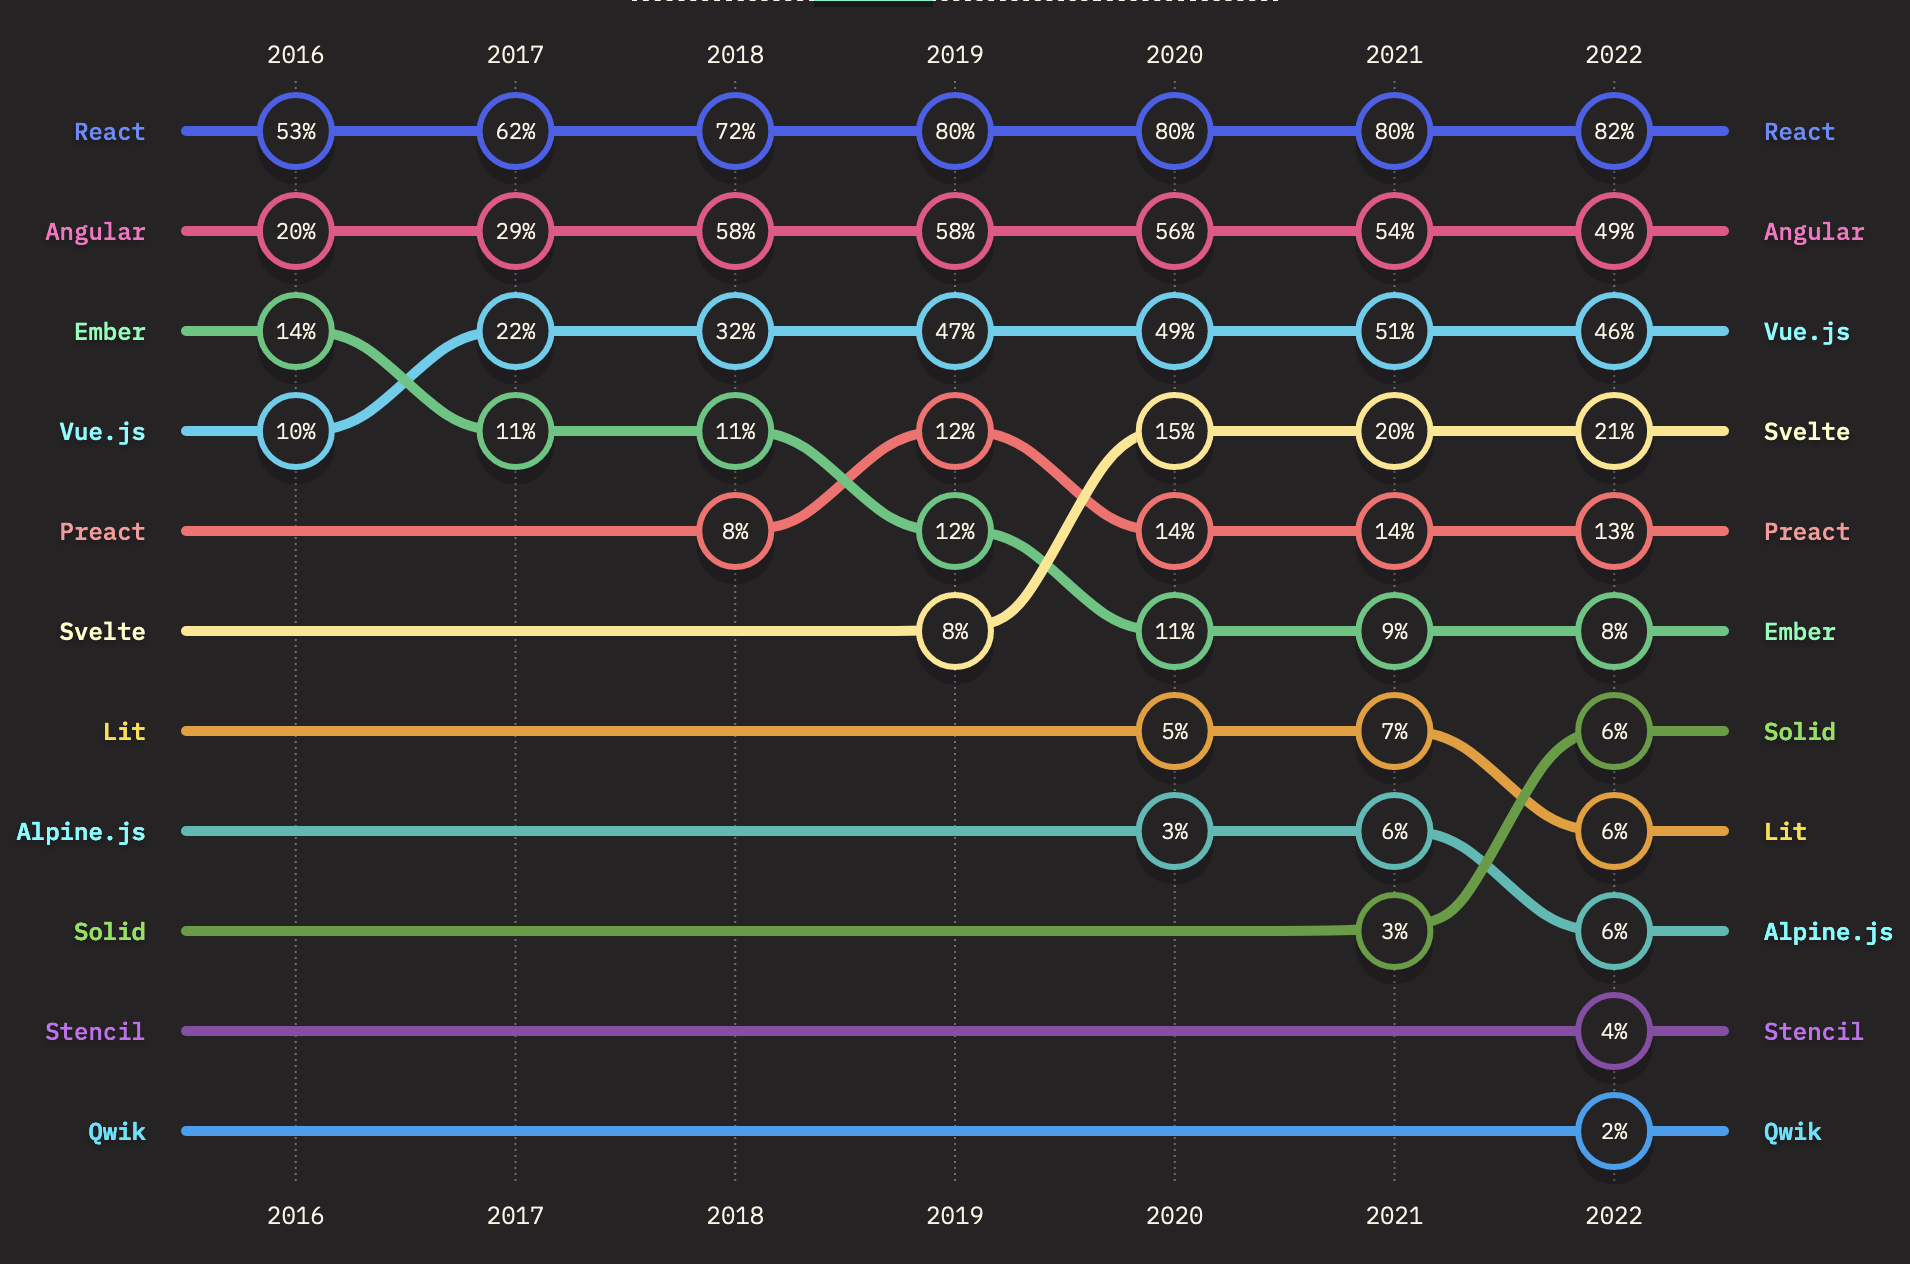
\includegraphics[scale=0.4]{04_Artefakte/01_Abbildungen/stateofjs-usage-frontend-frameworks-2022}
    \caption[Most used frontend frameworks in 2022]{State of JS: Most used frontend frameworks in 2022\protect\footnotemark}
    \label{fig:mostUsedFrameworks}
\end{figure}
\footnotetext{\cite{mostUsedFrontendFrameworks22}}

\subsection{React}

React (\url{https://react.dev/}), developed by Facebook and maintained by its successor Meta, has become the most widely used tool for building \ac{SPA}s and is steadily leading the rankings for most used frontend frameworks both in the Stack Overflow \parencite{stackOverflowPollWebFrameworks23} and the State Of JS \parencite{mostUsedFrontendFrameworks22} polls. By definition, it is not a framework but a \ac{UI} library that builds on other extensions to support state management, routing and deployment functionality. Although it is not a framework itself, there are existing frameworks like Next.js (\url{https://nextjs.org/}) for the web and ReactNative (\url{https://reactnative.dev/}) for building mobile apps using native functionality. React makes use of \ac{JSX}, which allows directly mixing inline \ac{HTML} with the \ac{JS} or \ac{TS} code structure.

\subsection{Vue}

Vue (\url{https://vuejs.org/}) was developed by Evan You and is maintained by an international team of individuals. It had a relatively marginal presence in the US and Europe in the first years after its inception. This can be partially attributed to its origin in China, as most of its supporting modules were localised in Chinese. Over the years, it grew in popularity and received much more international support, eventually overcoming the language barrier. Unlike React, it is billed as a "progressive framework" that provides fundamental functionality for building reactive components but also accommodates more complex use-cases \parencite{vueProgressiveFramework}. Vue builds on standard \ac{JS} or \ac{TS}, \ac{HTML} and \ac{CSS} to build components, recommending a simple template mechanism mixed with reactive substitutions. However, it also supports using \ac{JSX} for specifying inline \ac{HTML} within \ac{JS}. As with React, there are extensions and frameworks like Quasar (\url{https://quasar.dev/}) and Nuxt (\url{https://nuxt.com/}) that enable even more sophisticated workflows for application development and deployment.

\subsection{Angular}

Angular was initially released by Google in 2010 as AngularJS and officially discontinued in 2022 (\url{https://angularjs.org/}). A completely overhauled and currently used version 2 was released in 2016 and maintained by Google. It is different from React and Vue in that it is a complete framework that contains everything required to build and deploy an application, and it explicitly recommends \ac{TS} as a programming language. The framework is also less flexible in that it is opinionated and has its own set of best practices baked into the framework's structure.




\section{Backend frameworks}

\subsection{Express}

The Express JS framework provides the basic functionality to create web servers, including routing and middleware functionality. TJ Holowaychuk developed and sold it to StrongLoop, which IBM subsequently acquired. It is currently under the stewardship of the OpenJS Foundation.

Express has become the de facto standard for building web services in JS, leading the ranking in the State of JS survey \parencite{mostUsedBackendFrameworks22}. Although it contains the necessary parts to make a web service, it does not enforce a specific architecture, which can be problematic for maintaining a robust application structure. For developers who prefer a more explicit structure, various other frameworks are built on top of it that add more opinionated structures or extensions.

\subsection{Koa}

Billed as a successor to Express, Koa is developed by the team behind Express. It aims to provide a more robust and minimalistic iteration of the middleware-based architecture of Express. Like Express, it allows for building a service from scratch in free form but is also the basis for other, more explicitly structured frameworks.

Other frameworks and a more stringent and structured application structure might be more desirable for complex applications. There are numerous \ac{JS} frameworks, some based on Express or Koa, and others provide their own basis for routing. To review all possible options is beyond the scope of this study. In the following, three frameworks are selected for their specific nature related to popularity and stability, with an explicit focus on real-time applications.

\begin{table}[ht]
\centering
\caption{State of JS survey: Most used backend frameworks \parencite{mostUsedBackendFrameworks22}}
\label{tab:backendFrameworksRanking}
\begin{tabular}[t]{lcc}
\toprule
Framework & \% of question respondents\\
\midrule
Nest & 30.2\\
Feathers & 8.8\\
Meteor & 2.7\\
\bottomrule
\end{tabular}
\end{table}


\subsection{Nest}

Nest is a backend framework for developers who look for a more strictly opinionated and robust setup than Express, e.g. for enterprise applications. It follows a modular concept, making dependencies available to the services via injection. There are multiple database options, and transports can be HTTP and WebSockets. There are \ac{CLI} scripts that enable automatic generation of boilerplate application code, and the language used to build Nest applications is TypeScript. It ranks second among the most-used backend frameworks in the State of JS survey \parencite{mostUsedBackendFrameworks22}.

\subsection{Feathers}

This framework takes a different approach, making few assumptions about the specific application structure. It uses aspect-oriented programming and a service-centric architecture and before-, after- and around-hooks (so-called \textquote{cross-cutting concerns}) for the services that modify basic behaviour or add functionality. There are adapters for a wide range of databases and authentication methods. The framework has a dedicated concept of channels that enable real-time functionality and messaging to clients. Real-time transports are also abstracted and can be deployed using different WebSockets libraries. It also provides a \ac{CLI} to generate application code that can be written in \ac{JS} or \ac{TS}.

Feathers started as a hobby project by David Luecke and Eric Kryski in 2013 \parencite{feathersFrameworkHistory} and is currently maintained by David Luecke and a community of individual contributors. It still ranks in the lower percentages in the State of JS survey but almost doubled that percentage from the previous one in 2021 \parencite{mostUsedBackendFrameworks21}.

\subsection{Meteor}

Meteor focuses explicitly on real-time applications using WebSockets. The framework is a bit of an outlier in that its core is open-source, but other parts are proprietary code. Nonetheless, it should be mentioned because it has been around for over ten years and uses WebSockets exclusively. It was released in 2012 by a startup company, immediately received venture capital funding from Andreessen Horowitz and was eventually sold to Tiny Capital in 2019 \parencite{meteorSaleTinyCapital}.

The framework primarily uses MongoDB as a database system and initially provided its own package manager and ecosystem, build system, and template system based on Mustache. This exclusive strategy has been abandoned in favour of adopting the Node Package Manager. Still, it seems to be subject to debate regarding its ease of use versus its \textquote{growing pains} and related trouble with wide adoption \parencite{meteorDiscussionYCombinator}.


\section{Databases}

\subsection{MongoDB}

A document store database that is designed to hold large amounts of unstructured data. It has its own query language and features aggregation functionality that allows map/reduce and transformation operations or resolving of relations on the data before being sent to the client. Its focus on storing documents of any kind can become problematic since it can lead to inconsistent data very easily if appropriate care isn't applied in the application development (it supports schema validation, but that is not mandatory). However, this loose schematic handling can be beneficial if the application data can't be adequately modelled from the get-go and is subject to more frequent changes.

\subsection{PostgreSQL}

This very widely used database uses a table-based data topology and implements \ac{SQL} for interaction with the database and its contents. The relatively rigid database schema provides a more solid structure for data storage and retrieval but, on the other hand, requires migrations to be written to transition from one database structure version to another. This can become tedious if the data modelling process is continuously ongoing and volatile.



\section{Application deployment}

\subsection{Containerisation}

Containerisation, in the context of computing infrastructure, refers to the \textquote[\cite{containerisationDefinition}]{packaging of software code with just the operating system (OS) libraries and dependencies required to run the code to create a single lightweight executable—called a container—that runs consistently on any infrastructure.} It was popularised through the release of the Docker Engine, an open-source project devoted to creating an industry standard for application containerisation \parencite{dockerRelease}. The Docker team eventually launched the \ac{OCI} in 2015, which serves as \textquote{a lightweight, open governance structure (project), formed under the auspices of the Linux Foundation, for the express purpose of creating open industry standards around container formats and runtimes.} It subsequently received Docker's container runtime and format as a donation, which was released as runC version 1.0 in 2020 \parencite{openContainerInitiative}. Recently, it has become the de facto standard for packaging and delivering applications in the web development field and beyond. GitHub reports that \textquote[\cite{stateOfTheOctoverse23}]{in 2023, 4.3 million public and private repositories used Dockerfiles --- and more than 1 million public repositories used Dockerfiles for creating containers.}

\subsection{Container orchestration}

\textquote[\cite{orchestrationDefinition}]{Container orchestration automates the provisioning, deployment, networking, scaling, availability, and lifecycle management of containers.} The concept first gained popularity as Docker Swarm, which is a functionality of the Docker software, but its most successful instance so far is as the software package Kubernetes, which originated at Google in late 2013 \parencite{kubernetesHistory} and went on to be included in the \ac{CNCF}, a project by the Linux Foundation, that \textquote[\cite{cloudNativeComputingFoundation}]{aims to advance the state-of-the-art for building cloud-native applications and services}. It can be extended, highly customised and deployed on anything from an embedded device to a large-scale cloud infrastructure, providing a versatile deployment and management tool for many application infrastructures.
